\documentclass[12pt,a4paper]{article}

% ------------------------------------------------------------
% PACKAGES
% ------------------------------------------------------------
\usepackage[margin=1in]{geometry}
\usepackage{amsmath,amssymb,amsthm}
\usepackage{mathtools}
\usepackage{array}
\usepackage{booktabs}
\usepackage{enumitem}
\usepackage{float}
\usepackage{xcolor}
\usepackage{tikz}
\usepackage{tikz-3dplot}
\usepackage{pgfplots}
\usepackage{fancyhdr}
\usepackage{setspace}

\pgfplotsset{compat=1.18}

% ------------------------------------------------------------
% DOCUMENT SETTINGS
% ------------------------------------------------------------
\onehalfspacing

\pagestyle{fancy}
\fancyhf{}
\lhead{APM1220 -- FA 2}
\rhead{Foundations}
\cfoot{\thepage}

\setlength{\parindent}{0pt}
\setlength{\parskip}{6pt}

% ------------------------------------------------------------
% CUSTOM COMMANDS
% ------------------------------------------------------------
\newcommand{\R}{\mathbb{R}}
\newcommand{\xbar}{\overline{\mathbf{x}}}
\newcommand{\one}{\mathbf{1}}
\newcommand{\Smat}{\mathbf{S}}
\newcommand{\Rmat}{\mathbf{R}}

% ------------------------------------------------------------
% TITLE
% ------------------------------------------------------------
\begin{document}

\begin{titlepage}
    \centering
    \vspace*{1.5cm}

    {\Large\textbf{APM1220}}\\[0.5cm]
    {\LARGE\textbf{Formative Assessment 2}}\\[1cm]

\end{titlepage}
\newpage

\section{Problem 3.1}

Given the data matrix
\[
X=
\begin{bmatrix}
9&1\\
5&3\\
1&2
\end{bmatrix},
\]
we have \(n=3\) observations and \(p=2\) variables.

The two variable vectors are
\[
\mathbf{y}_1=
\begin{bmatrix}
9\\5\\1
\end{bmatrix},
\qquad
\mathbf{y}_2=
\begin{bmatrix}
1\\3\\2
\end{bmatrix}.
\]

% ------------------------------------------------------------
\subsection*{(a) Scatter plot and sample mean}

The sample mean vector is
\[
\overline{\mathbf{x}}
=
\begin{bmatrix}
\overline{x}_1\\
\overline{x}_2
\end{bmatrix}
=
\begin{bmatrix}
\dfrac{9+5+1}{3}\\[6pt]
\dfrac{1+3+2}{3}
\end{bmatrix}
=
\begin{bmatrix}
5\\
2
\end{bmatrix}.
\]

Thus, the three observations are
\[
(9,1),\qquad (5,3),\qquad (1,2),
\]
and the sample mean is located at
\[
\boxed{(5,2)}.
\]

The scatter plot is shown below.

\begin{figure}[H]
\centering
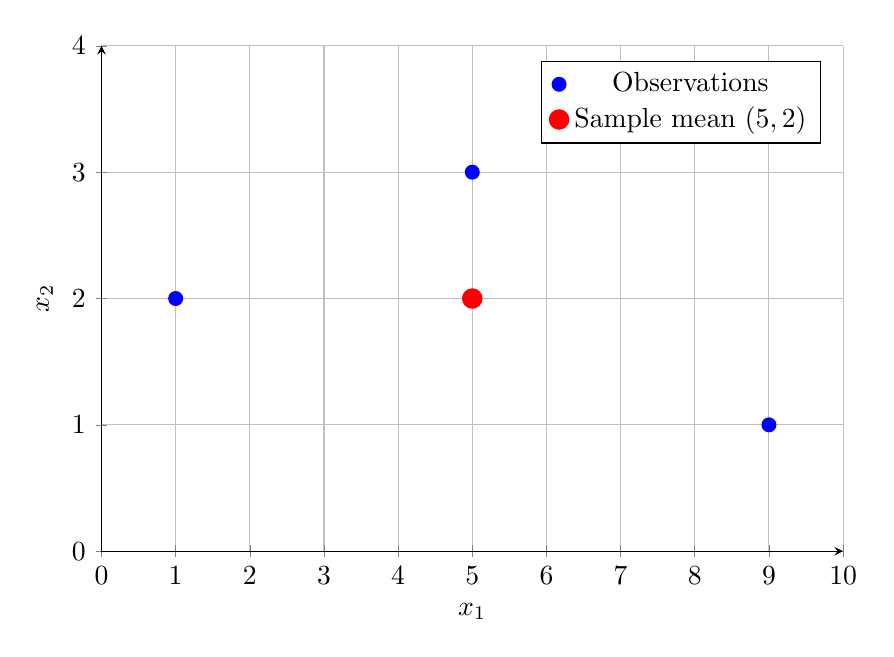
\begin{tikzpicture}
\begin{axis}[
    width=11cm,
    height=8cm,
    xmin=0,xmax=10,
    ymin=0,ymax=4,
    xlabel={$x_1$},
    ylabel={$x_2$},
    grid=both,
    axis lines=left,
    xtick={0,1,...,10},
    ytick={0,1,2,3,4},
    legend style={at={(0.97,0.97)},anchor=north east}
]
\addplot[
    only marks,
    mark=*,
    mark size=2.5pt,
    blue
] coordinates {
    (9,1)
    (5,3)
    (1,2)
};
\addlegendentry{Observations}

\addplot[
    only marks,
    mark=*,
    mark size=3.5pt,
    red
] coordinates {(5,2)};
\addlegendentry{Sample mean $(5,2)$}

\end{axis}
\end{tikzpicture}
\caption{Scatter plot of the two-dimensional observations.}
\end{figure}

Therefore,
\[
\boxed{\overline{\mathbf{x}}=(5,2)'}.
\]

% ------------------------------------------------------------
\subsection*{(b) Three-dimensional representation and deviation vectors}

The mean of the first variable is
\[
\overline{x}_1=5,
\]
so
\[
\overline{x}_1\mathbf{1}
=
\begin{bmatrix}
5\\5\\5
\end{bmatrix}.
\]

The deviation vector for the first variable is therefore
\[
\mathbf{y}_1-\overline{x}_1\mathbf{1}
=
\begin{bmatrix}
9\\5\\1
\end{bmatrix}
-
\begin{bmatrix}
5\\5\\5
\end{bmatrix}
=
\boxed{
\begin{bmatrix}
4\\0\\-4
\end{bmatrix}}.
\]

Similarly,
\[
\overline{x}_2=2,
\]
so
\[
\overline{x}_2\mathbf{1}
=
\begin{bmatrix}
2\\2\\2
\end{bmatrix},
\]
and
\[
\mathbf{y}_2-\overline{x}_2\mathbf{1}
=
\begin{bmatrix}
1\\3\\2
\end{bmatrix}
-
\begin{bmatrix}
2\\2\\2
\end{bmatrix}
=
\boxed{
\begin{bmatrix}
-1\\1\\0
\end{bmatrix}}.
\]

Thus, in the three-dimensional observation space,
\[
\boxed{
\mathbf{d}_1=
\begin{bmatrix}
4\\0\\-4
\end{bmatrix},
\qquad
\mathbf{d}_2=
\begin{bmatrix}
-1\\1\\0
\end{bmatrix}.
}
\]

Both deviation vectors have components summing to zero:
\[
4+0-4=0,
\qquad
-1+1+0=0.
\]
Hence both vectors lie in the plane
\[
z_1+z_2+z_3=0.
\]

A three-dimensional sketch is given below.

\begin{figure}[H]
\centering
\tdplotsetmaincoords{70}{120}
\begin{tikzpicture}[tdplot_main_coords,scale=0.8]

% Axes
\draw[->,thick] (0,0,0) -- (5,0,0) node[anchor=north east] {$z_1$};
\draw[->,thick] (0,0,0) -- (0,4,0) node[anchor=north west] {$z_2$};
\draw[->,thick] (0,0,0) -- (0,0,5) node[anchor=south] {$z_3$};

% Vector d1
\draw[->,very thick,blue] (0,0,0) -- (4,0,-4)
    node[midway,above] {$\mathbf{d}_1=(4,0,-4)$};

% Vector d2
\draw[->,very thick,red] (0,0,0) -- (-1,1,0)
    node[midway,above] {$\mathbf{d}_2=(-1,1,0)$};

% Endpoints
\filldraw[blue] (4,0,-4) circle (2pt);
\filldraw[red] (-1,1,0) circle (2pt);

% Origin
\node[below left] at (0,0,0) {$O$};

\end{tikzpicture}
\caption{Three-dimensional representation of the deviation vectors.}
\end{figure}

% ------------------------------------------------------------
\subsection*{(c) Lengths, angle, \(S_n\), and \(R\)}

The length of the first deviation vector is
\[
\|\mathbf{d}_1\|
=
\sqrt{4^2+0^2+(-4)^2}
=
\sqrt{32}
=
\boxed{4\sqrt{2}}.
\]

The length of the second deviation vector is
\[
\|\mathbf{d}_2\|
=
\sqrt{(-1)^2+1^2+0^2}
=
\sqrt{2}.
\]
Hence
\[
\boxed{\|\mathbf{d}_2\|=\sqrt{2}}.
\]

The dot product is
\[
\mathbf{d}_1'\mathbf{d}_2
=
(4)(-1)+(0)(1)+(-4)(0)
=
-4.
\]

Therefore, the cosine of the angle \(\theta\) between the two vectors is
\[
\cos\theta
=
\frac{\mathbf{d}_1'\mathbf{d}_2}
{\|\mathbf{d}_1\|\|\mathbf{d}_2\|}
=
\frac{-4}{(4\sqrt{2})(\sqrt{2})}
=
\frac{-4}{8}
=
\boxed{-\frac12}.
\]

Thus,
\[
\boxed{\theta=120^\circ}.
\]

The centered data matrix is
\[
X-\one\xbar'
=
\begin{bmatrix}
4&-1\\
0&1\\
-4&0
\end{bmatrix}.
\]

The covariance matrix using divisor \(n\) is
\[
S_n
=
\frac{1}{n}
(X-\one\xbar')'
(X-\one\xbar').
\]

Since
\[
(X-\one\xbar')'
(X-\one\xbar')
=
\begin{bmatrix}
32&-4\\
-4&2
\end{bmatrix},
\]
we obtain
\[
S_n
=
\frac13
\begin{bmatrix}
32&-4\\
-4&2
\end{bmatrix}
=
\boxed{
\begin{bmatrix}
\dfrac{32}{3}&-\dfrac43\\[4pt]
-\dfrac43&\dfrac23
\end{bmatrix}}.
\]

The usual sample covariance matrix, using divisor \(n-1=2\), is
\[
S
=
\frac12
\begin{bmatrix}
32&-4\\
-4&2
\end{bmatrix}
=
\boxed{
\begin{bmatrix}
16&-2\\
-2&1
\end{bmatrix}}.
\]

The correlation matrix is
\[
R=
\begin{bmatrix}
1&r_{12}\\
r_{12}&1
\end{bmatrix},
\]
where
\[
r_{12}
=
\frac{s_{12}}{\sqrt{s_{11}s_{22}}}
=
\frac{-2}{\sqrt{16(1)}}
=
-\frac12.
\]

Thus,
\[
\boxed{
R=
\begin{bmatrix}
1&-\dfrac12\\[4pt]
-\dfrac12&1
\end{bmatrix}}.
\]

Notice that the cosine calculated from the deviation vectors is exactly the sample correlation:
\[
\boxed{\cos\theta=r_{12}=-\frac12}.
\]

The squared lengths of the deviation vectors are related to the diagonal entries of the scatter/covariance matrix:
\[
\|\mathbf{d}_1\|^2=32,
\qquad
\|\mathbf{d}_2\|^2=2.
\]
After dividing by \(n-1\),
\[
s_{11}=\frac{32}{2}=16,
\qquad
s_{22}=\frac{2}{2}=1.
\]

Therefore, the lengths describe the amount of variation in each variable, while the angle describes their correlation.

\[
\boxed{\text{Longer deviation vectors correspond to greater variance, while the angle determines the correlation.}}
\]

% ============================================================
% PROBLEM 3.6
% ============================================================
\newpage
\section{Problem 3.6}

Consider
\[
X=
\begin{bmatrix}
-1&3&-2\\
2&4&2\\
5&2&3
\end{bmatrix}.
\]

% ------------------------------------------------------------
\subsection*{(a) Matrix of deviations and rank}

First calculate the sample mean vector:
\[
\overline{\mathbf{x}}
=
\begin{bmatrix}
\dfrac{-1+2+5}{3}\\[6pt]
\dfrac{3+4+2}{3}\\[6pt]
\dfrac{-2+2+3}{3}
\end{bmatrix}
=
\begin{bmatrix}
2\\3\\1
\end{bmatrix}.
\]

Hence
\[
\one\overline{\mathbf{x}}'
=
\begin{bmatrix}
2&3&1\\
2&3&1\\
2&3&1
\end{bmatrix}.
\]

The deviation matrix is
\[
X-\one\overline{\mathbf{x}}'
=
\begin{bmatrix}
-1&3&-2\\
2&4&2\\
5&2&3
\end{bmatrix}
-
\begin{bmatrix}
2&3&1\\
2&3&1\\
2&3&1
\end{bmatrix},
\]
so
\[
\boxed{
X-\one\overline{\mathbf{x}}'
=
\begin{bmatrix}
-3&0&-3\\
0&1&1\\
3&-1&2
\end{bmatrix}}.
\]

Let the columns of this matrix be \(\mathbf{d}_1,\mathbf{d}_2,\mathbf{d}_3\). Then
\[
\mathbf{d}_1=
\begin{bmatrix}
-3\\0\\3
\end{bmatrix},
\qquad
\mathbf{d}_2=
\begin{bmatrix}
0\\1\\-1
\end{bmatrix},
\]
and
\[
\mathbf{d}_3=
\begin{bmatrix}
-3\\1\\2
\end{bmatrix}.
\]

Observe that
\[
\mathbf{d}_1+\mathbf{d}_2
=
\begin{bmatrix}
-3\\0\\3
\end{bmatrix}
+
\begin{bmatrix}
0\\1\\-1
\end{bmatrix}
=
\begin{bmatrix}
-3\\1\\2
\end{bmatrix}
=
\mathbf{d}_3.
\]

Therefore, the third column is a linear combination of the first two:
\[
\boxed{\mathbf{d}_3=\mathbf{d}_1+\mathbf{d}_2}.
\]

Thus the columns are linearly dependent, and
\[
\boxed{\operatorname{rank}(X-\one\overline{\mathbf{x}}')=2}.
\]

In particular, the deviation matrix is \emph{not} of full rank.

% ------------------------------------------------------------
\subsection*{(b) Covariance matrix and generalized variance}

The sample covariance matrix is
\[
S
=
\frac{1}{n-1}
(X-\one\overline{\mathbf{x}}')'
(X-\one\overline{\mathbf{x}}').
\]

Here \(n=3\), so
\[
S
=
\frac12
\begin{bmatrix}
-3&0&3\\
0&1&-1\\
-3&1&2
\end{bmatrix}
\begin{bmatrix}
-3&0&-3\\
0&1&1\\
3&-1&2
\end{bmatrix}.
\]

The cross-product matrix is
\[
(X-\one\overline{\mathbf{x}}')'
(X-\one\overline{\mathbf{x}}')
=
\begin{bmatrix}
18&-3&15\\
-3&2&-1\\
15&-1&14
\end{bmatrix}.
\]

Therefore,
\[
\boxed{
S=
\begin{bmatrix}
9&-\dfrac32&\dfrac{15}{2}\\[5pt]
-\dfrac32&1&-\dfrac12\\[5pt]
\dfrac{15}{2}&-\dfrac12&7
\end{bmatrix}}.
\]

The generalized sample variance is
\[
|S|=\det(S).
\]

Thus,
\[
\begin{aligned}
|S|
&=
\begin{vmatrix}
9&-\frac32&\frac{15}{2}\\
-\frac32&1&-\frac12\\
\frac{15}{2}&-\frac12&7
\end{vmatrix}\\[4pt]
&=0.
\end{aligned}
\]

Hence,
\[
\boxed{|S|=0}.
\]

This agrees with the fact that the columns of the deviation matrix are linearly dependent.

Geometrically, the generalized variance is proportional to the squared volume of the covariance ellipsoid. Since the variables are linearly dependent, the observations do not occupy a full three-dimensional volume. Instead, they lie in a lower-dimensional subspace.

Therefore,
\[
\boxed{\text{The generalized variance is zero because the covariance ellipsoid has zero three-dimensional volume.}}
\]

% ------------------------------------------------------------
\subsection*{(c) Total sample variance}

The total sample variance is the sum of the individual sample variances, equivalently the trace of \(S\):
\[
\operatorname{tr}(S)
=
s_{11}+s_{22}+s_{33}.
\]

Therefore,
\[
\operatorname{tr}(S)
=
9+1+7
=
\boxed{17}.
\]

Thus the total sample variance is
\[
\boxed{17}.
\]

% ============================================================
% PROBLEM 3.9
% ============================================================
\newpage
\section{Problem 3.9}

The data matrix is
\[
X=
\begin{bmatrix}
12&17&29\\
18&20&38\\
14&16&30\\
20&18&38\\
16&19&35
\end{bmatrix}.
\]

% ------------------------------------------------------------
\subsection*{(a) Mean-corrected data matrix and linear dependence}

The sample means are
\[
\overline{x}_1
=
\frac{12+18+14+20+16}{5}
=
16,
\]
\[
\overline{x}_2
=
\frac{17+20+16+18+19}{5}
=
18,
\]
and
\[
\overline{x}_3
=
\frac{29+38+30+38+35}{5}
=
34.
\]

Hence
\[
\overline{\mathbf{x}}
=
\begin{bmatrix}
16\\18\\34
\end{bmatrix}.
\]

The mean-corrected matrix is
\[
X-\one\overline{\mathbf{x}}'
=
\begin{bmatrix}
12-16&17-18&29-34\\
18-16&20-18&38-34\\
14-16&16-18&30-34\\
20-16&18-18&38-34\\
16-16&19-18&35-34
\end{bmatrix}.
\]

Therefore,
\[
\boxed{
X-\one\overline{\mathbf{x}}'
=
\begin{bmatrix}
-4&-1&-5\\
2&2&4\\
-2&-2&-4\\
4&0&4\\
0&1&1
\end{bmatrix}}.
\]

Let the three columns be \(\mathbf{d}_1,\mathbf{d}_2,\mathbf{d}_3\). We observe that
\[
\mathbf{d}_3=\mathbf{d}_1+\mathbf{d}_2.
\]

Indeed,
\[
\begin{bmatrix}
-4\\2\\-2\\4\\0
\end{bmatrix}
+
\begin{bmatrix}
-1\\2\\-2\\0\\1
\end{bmatrix}
=
\begin{bmatrix}
-5\\4\\-4\\4\\1
\end{bmatrix}
=
\mathbf{d}_3.
\]

Therefore,
\[
\mathbf{d}_1+\mathbf{d}_2-\mathbf{d}_3=\mathbf{0}.
\]

A vector establishing the linear dependence is therefore
\[
\boxed{
\mathbf{a}
=
\begin{bmatrix}
1\\1\\-1
\end{bmatrix}}.
\]

Equivalently,
\[
\boxed{a'=[1,1,-1]}.
\]

% ------------------------------------------------------------
\subsection*{(b) Sample covariance matrix, generalized variance, and \(Sa=0\)}

The sample covariance matrix is
\[
S
=
\frac{1}{n-1}
(X-\one\overline{\mathbf{x}}')'
(X-\one\overline{\mathbf{x}}').
\]

Since \(n=5\),
\[
S
=
\frac14
(X-\one\overline{\mathbf{x}}')'
(X-\one\overline{\mathbf{x}}').
\]

The cross-product matrix is
\[
(X-\one\overline{\mathbf{x}}')'
(X-\one\overline{\mathbf{x}}')
=
\begin{bmatrix}
40&12&52\\
12&10&22\\
52&22&74
\end{bmatrix}.
\]

Hence
\[
\boxed{
S=
\begin{bmatrix}
10&3&13\\
3&\dfrac52&\dfrac{11}{2}\\
13&\dfrac{11}{2}&\dfrac{37}{2}
\end{bmatrix}}.
\]

The generalized variance is
\[
|S|=\det(S).
\]

Since the columns are linearly dependent, the determinant must be zero. Directly,
\[
\boxed{|S|=0}.
\]

Now verify that
\[
S\mathbf{a}=\mathbf{0}.
\]

We have
\[
S
\begin{bmatrix}
1\\1\\-1
\end{bmatrix}
=
\begin{bmatrix}
10&3&13\\
3&\frac52&\frac{11}{2}\\
13&\frac{11}{2}&\frac{37}{2}
\end{bmatrix}
\begin{bmatrix}
1\\1\\-1
\end{bmatrix}.
\]

The first component is
\[
10+3-13=0.
\]

The second component is
\[
3+\frac52-\frac{11}{2}
=
3-\!3
=
0.
\]

The third component is
\[
13+\frac{11}{2}-\frac{37}{2}
=
13-\!13
=
0.
\]

Therefore,
\[
\boxed{
S\mathbf{a}
=
\begin{bmatrix}
0\\0\\0
\end{bmatrix}}.
\]

Thus \(\mathbf{a}\) belongs to the null space of \(S\), and because \(S\) is symmetric, it can be rescaled to give an eigenvector associated with eigenvalue \(0\).

For example, the unit eigenvector is
\[
\boxed{
\frac{1}{\sqrt3}
\begin{bmatrix}
1\\1\\-1
\end{bmatrix}}
\]
with eigenvalue
\[
\boxed{\lambda=0}.
\]

% ------------------------------------------------------------
\subsection*{(c) Verification using the original data matrix}

Consider the first two columns:
\[
x_1=
\begin{bmatrix}
12\\18\\14\\20\\16
\end{bmatrix},
\qquad
x_2=
\begin{bmatrix}
17\\20\\16\\18\\19
\end{bmatrix}.
\]

Their sum is
\[
x_1+x_2
=
\begin{bmatrix}
12+17\\
18+20\\
14+16\\
20+18\\
16+19
\end{bmatrix}
=
\begin{bmatrix}
29\\38\\30\\38\\35
\end{bmatrix}.
\]

But this is exactly the third column:
\[
x_3=
\begin{bmatrix}
29\\38\\30\\38\\35
\end{bmatrix}.
\]

Therefore,
\[
\boxed{x_3=x_1+x_2}.
\]

Rearranging,
\[
x_1+x_2-x_3=0.
\]

Thus the linear dependence is established by
\[
\boxed{a_1=1,\qquad a_2=1,\qquad a_3=-1}.
\]

% ============================================================
% PROBLEM 3.18
% ============================================================
\newpage
\section{Problem 3.18}

The mean vector is
\[
\overline{\mathbf{x}}
=
\begin{bmatrix}
0.766\\
0.508\\
0.438\\
0.161
\end{bmatrix},
\]
and the covariance matrix is
\[
S=
\begin{bmatrix}
0.856&0.635&0.173&0.096\\
0.635&0.568&0.128&0.067\\
0.173&0.127&0.171&0.039\\
0.096&0.067&0.039&0.043
\end{bmatrix}.
\]

For a linear combination
\[
z=\mathbf{a}'\mathbf{x},
\]
the sample mean and variance are
\[
\overline{z}=\mathbf{a}'\overline{\mathbf{x}},
\qquad
s_z^2=\mathbf{a}'S\mathbf{a}.
\]

% ------------------------------------------------------------
\subsection*{(a) Total energy consumption}

Let the total energy consumption be
\[
T=x_1+x_2+x_3+x_4.
\]

Therefore,
\[
T=\mathbf{a}'\mathbf{x},
\qquad
\mathbf{a}
=
\begin{bmatrix}
1\\1\\1\\1
\end{bmatrix}.
\]

The sample mean is
\[
\overline{T}
=
\mathbf{a}'\overline{\mathbf{x}}.
\]

Thus,
\[
\begin{aligned}
\overline{T}
&=
0.766+0.508+0.438+0.161\\
&=
\boxed{1.873}.
\end{aligned}
\]

Now calculate the variance:
\[
s_T^2=\mathbf{a}'S\mathbf{a}.
\]

This is equivalent to summing every element of \(S\):
\[
\begin{aligned}
s_T^2
={}&
0.856+0.635+0.173+0.096\\
&+0.635+0.568+0.128+0.067\\
&+0.173+0.127+0.171+0.039\\
&+0.096+0.067+0.039+0.043.
\end{aligned}
\]

Therefore,
\[
\boxed{s_T^2=3.912}.
\]

Hence the total energy consumption has
\[
\boxed{\text{sample mean}=1.873}
\]
and
\[
\boxed{\text{sample variance}=3.912}.
\]

% ------------------------------------------------------------
\subsection*{(b) Excess petroleum consumption over natural gas}

Define
\[
D=x_1-x_2.
\]

Thus,
\[
D=\mathbf{c}'\mathbf{x},
\qquad
\mathbf{c}
=
\begin{bmatrix}
1\\-1\\0\\0
\end{bmatrix}.
\]

The sample mean is
\[
\overline{D}
=
\mathbf{c}'\overline{\mathbf{x}}
=
0.766-0.508
=
\boxed{0.258}.
\]

The variance is
\[
s_D^2=\mathbf{c}'S\mathbf{c}.
\]

Therefore,
\[
\begin{aligned}
s_D^2
&=
s_{11}+s_{22}-2s_{12}\\
&=
0.856+0.568-2(0.635)\\
&=
1.424-1.270\\
&=
\boxed{0.154}.
\end{aligned}
\]

Hence,
\[
\boxed{\overline{D}=0.258},
\qquad
\boxed{s_D^2=0.154}.
\]

Now find the covariance between \(D\) and the total variable \(T\).

Since
\[
T=\mathbf{a}'\mathbf{x},
\qquad
D=\mathbf{c}'\mathbf{x},
\]
the covariance is
\[
s_{DT}=\mathbf{c}'S\mathbf{a}.
\]

First calculate
\[
S\mathbf{a}
=
\begin{bmatrix}
0.856+0.635+0.173+0.096\\
0.635+0.568+0.128+0.067\\
0.173+0.127+0.171+0.039\\
0.096+0.067+0.039+0.043
\end{bmatrix}
=
\begin{bmatrix}
1.760\\
1.398\\
0.510\\
0.245
\end{bmatrix}.
\]

Therefore,
\[
\begin{aligned}
s_{DT}
&=
\begin{bmatrix}
1&-1&0&0
\end{bmatrix}
\begin{bmatrix}
1.760\\
1.398\\
0.510\\
0.245
\end{bmatrix}\\
&=
1.760-1.398\\
&=
\boxed{0.362}.
\end{aligned}
\]

Thus,
\[
\boxed{\operatorname{Cov}(D,T)=0.362}.
\]

% ============================================================
% PROBLEM 3.20
% ============================================================
\newpage
\section{Problem 3.20}

The 25 observations are given below.

\begin{table}[H]
\centering
\small
\begin{tabular}{ccc}
\toprule
$x_1$ & $x_2$ & $x_2-x_1$\\
\midrule
12.5 & 13.7 & 1.2\\
14.5 & 16.5 & 2.0\\
8.0 & 17.4 & 9.4\\
9.0 & 11.0 & 2.0\\
19.5 & 23.6 & 4.1\\
8.0 & 13.2 & 5.2\\
9.0 & 32.1 & 23.1\\
7.0 & 12.3 & 5.3\\
7.0 & 11.8 & 4.8\\
9.0 & 24.4 & 15.4\\
6.5 & 18.2 & 11.7\\
10.5 & 22.0 & 11.5\\
10.0 & 32.5 & 22.5\\
4.5 & 18.7 & 14.2\\
7.0 & 15.8 & 8.8\\
8.5 & 15.6 & 7.1\\
6.5 & 12.0 & 5.5\\
8.0 & 12.8 & 4.8\\
3.5 & 26.1 & 22.6\\
8.0 & 14.5 & 6.5\\
17.5 & 42.3 & 24.8\\
10.5 & 17.5 & 7.0\\
12.0 & 21.8 & 9.8\\
6.0 & 10.4 & 4.4\\
13.0 & 25.6 & 12.6\\
\bottomrule
\end{tabular}
\caption{Snow data and individual differences.}
\end{table}

% ------------------------------------------------------------
\subsection*{(a) Mean and variance of \(x_2-x_1\) using summary statistics}

Let
\[
D=x_2-x_1.
\]

We first calculate the summary statistics of \(x_1\) and \(x_2\).

For \(x_1\),
\[
\sum_{j=1}^{25}x_{j1}=235.5,
\]
so
\[
\overline{x}_1
=
\frac{235.5}{25}
=
\boxed{9.42}.
\]

Also,
\[
\sum_{j=1}^{25}x_{j1}^2=2557.75.
\]

Therefore,
\[
\begin{aligned}
s_{11}
&=
\frac{
\sum x_{j1}^2
-\dfrac{(\sum x_{j1})^2}{n}
}{n-1}\\
&=
\frac{
2557.75-\dfrac{(235.5)^2}{25}
}{24}\\
&=
\frac{339.34}{24}\\
&=
\boxed{\frac{16967}{1200}}
\approx 14.1392.
\end{aligned}
\]

For \(x_2\),
\[
\sum_{j=1}^{25}x_{j2}=481.8,
\]
so
\[
\overline{x}_2
=
\frac{481.8}{25}
=
\boxed{19.272}.
\]

Also,
\[
\sum_{j=1}^{25}x_{j2}^2=10778.98.
\]

Thus,
\[
\begin{aligned}
s_{22}
&=
\frac{
10778.98-\dfrac{(481.8)^2}{25}
}{24}\\
&=
\boxed{\frac{1867163}{30000}}
\approx 62.2388.
\end{aligned}
\]

The cross-product sum is
\[
\sum_{j=1}^{25}x_{j1}x_{j2}=4861.90.
\]

Therefore,
\[
\begin{aligned}
s_{12}
&=
\frac{
\sum x_{j1}x_{j2}
-\dfrac{(\sum x_{j1})(\sum x_{j2})}{n}
}{n-1}\\
&=
\frac{
4861.90-\dfrac{(235.5)(481.8)}{25}
}{24}\\
&=
\boxed{\frac{20209}{1500}}
\approx 13.4727.
\end{aligned}
\]

The mean of the difference is
\[
\begin{aligned}
\overline{D}
&=
\overline{x}_2-\overline{x}_1\\
&=
19.272-9.42\\
&=
\boxed{9.852}.
\end{aligned}
\]

The variance of a difference is
\[
s_D^2
=
s_{22}+s_{11}-2s_{12}.
\]

Therefore,
\[
\begin{aligned}
s_D^2
&=
62.2387667+14.1391667
-2(13.4726667)\\
&=
\boxed{49.4326}.
\end{aligned}
\]

In exact fractional form,
\[
\boxed{
s_D^2=\frac{247163}{5000}.
}
\]

Thus, using the summary statistics,
\[
\boxed{
\overline{x_2-x_1}=9.852,
\qquad
s_{x_2-x_1}^2=49.4326.
}
\]

% ------------------------------------------------------------
\subsection*{(b) Mean and variance using the individual differences}

The individual differences are
\[
\begin{aligned}
d_j=x_{j2}-x_{j1}
={}&
1.2,\;2.0,\;9.4,\;2.0,\;4.1,\;5.2,\;23.1,\;5.3,\;4.8,\\
&15.4,\;11.7,\;11.5,\;22.5,\;14.2,\;8.8,\;7.1,\;5.5,\;4.8,\\
&22.6,\;6.5,\;24.8,\;7.0,\;9.8,\;4.4,\;12.6.
\end{aligned}
\]

Their sum is
\[
\sum_{j=1}^{25}d_j=246.3,
\]
and hence
\[
\overline{d}
=
\frac{246.3}{25}
=
\boxed{9.852}.
\]

The sum of squared differences is
\[
\sum_{j=1}^{25}d_j^2=3612.93.
\]

Therefore, the sample variance is
\[
\begin{aligned}
s_d^2
&=
\frac{
\sum d_j^2-\dfrac{(\sum d_j)^2}{n}
}{n-1}\\
&=
\frac{
3612.93-\dfrac{(246.3)^2}{25}
}{24}\\
&=
\frac{1186.3824}{24}\\
&=
\boxed{49.4326}.
\end{aligned}
\]

Thus,
\[
\boxed{
\overline{d}=9.852,
\qquad
s_d^2=49.4326.
}
\]

Comparing the results from parts (a) and (b),
\[
\boxed{
\overline{x_2-x_1}=9.852
}
\]
and
\[
\boxed{
s_{x_2-x_1}^2=49.4326
}
\]
using both methods.

Therefore, the two approaches give exactly the same results, as expected.

\end{document}
```

